\section{緒言}

\subsection{研究背景}

一般的に,流体はせん断応力がせん断速度に比例するNewton流体と,せん断応力がせん断速度が非線形となる非Newton流体に分類することができる.

Fig.\ref{fig:1-fluid-curve}に示す通り,Newton流体はせん断速度とせん断応力が比例関係にある流体である.一方でそれ以外の流体は非Newton流体と呼ばれている.非Newton流体はDilatant fluid, Pseudoplastic, Bingham plastic, Viscoplastic が挙げられている.
非Newton流体のうち,Bingham plastic 流体, Viscoplastic 流体はせん断応力がある一定になるまでせん断速度が発生しない流体である.一方で,Dilatant fluid 流体, Pseudoplastic 流体はせん断応力が少しでも加わると,せん断速度が発生し流体的挙動を示す.これら非Newton流体の粘度を示す理論として,Power-law model (Ostwald-De Waele model), Cross model,Carreau viscosity equationやHerschel-Bulkley modelなどを挙げることができる\cite{ref:1}.Power-law model はせん断速度の限られた範囲内にて適応することができる.理論式中の指数によってNewton流体,shear-thinning流体と,shear-thickening流体に分類することができる.これらのせん断速度と粘度の関係性はFig.\ref{fig:2-Newton-fluid}に示す通りである.これら2種類の流体のうち,本研究で扱うshear-thinning流体は,せん断速度$\dot{\gamma}$が高くなるほど粘度$\mu$が低くなる性質を有している.この流体は擬塑性流体とも呼ばれている.

Cross modelはshear-thinning性が構造的に引き起こされるといった仮説において導き出された理論である.これは広いせん断速度において適用することができる.また,Carreau viscosity equationはCross modelをpower-law領域においてより適合するよう修正したものとなっている.Herschel-Bulkley modelはBingham plasticやViscoplasticといった静止状態の流体においてせん断応力が存在する流体を示す理論となっている\cite{ref:1}.

擬塑性流体とは,液状で巨大な分子が存在する流体や固体粒子が懸濁状で液体に存在する流体のことである.擬塑性流体の一般的な例として,砂や砂利など粒状の物質と水が混合する,泥流や雪崩といった自然現象を挙げることができる.また,産業分野において,擬塑性流体を混合や輸送行うことがある.効率よく輸送や混合を行うためには,せん断速度が高くなるほど粘度が低くなる性質を活かし,粘性による抵抗の低減を図る必要がある.

例えば,Ohta {\it et al.} \cite{ref:2}は非弾性擬塑性流体中における液滴の上昇運動に対し,液滴周りのせん断速度による粘度低下があたえる影響を明らかにした.加えて,Ohta {\it et al.} \cite{ref:3}は液滴周りの粘度分布を数値計算より求め,局所的な粘度低下は液滴の形状に大きく依存することを明らかにした.また,Zhang {\it et al.} \cite{ref:4}は非弾性擬塑性流体中における単一気泡の上昇運動に対し,数値計算,実験から,気泡周囲のせん断速度,粘度,速度場を明らかにした.

超音波振動の影響による抵抗低下に関してvan den Wildenberg {\it et al.}\cite{ref:6}による研究があげられる.本研究では,粒子の上部を水で満たした容器ごと振動させ,その粒子中に球を落下させた.その結果をFig.\ref{fig:4-sinking}に示す.Fig.\ref{fig:4-sinking}(a1)において,$\Gamma$は振動強度である.振動によって落下球表面におけるせん断応力が減少し,振動強度を強くするとより深くまで沈降すると報告された.Iwata {\it et al.}\cite{ref:5}は,超音波振動によって擬塑性流体中における気泡の体積を周期的に増加・減少させることにより,気泡近傍の局所せん断粘度を低下し,上昇速度が増加することを明らかにした.これは気泡の膨張収縮により,気泡近傍に強い局所せん断流れが生じるためである.また,Iwamuro \textit{et al}.\cite{ref:8}では擬塑性流体中を落下する球に超音波振動を照射し,高速化のメカニズムに関して,流体物性,物体形状,超音波強度および周波数を変化させることで調査が行われた.この結果,球の落下には弾性,粘性の関係が大きく関わることが分かった.また,球の落下速度の高速化には,音響境界層粘度および厚さに速度比が相関しており,音響境界層の形成が影響を及ぼしていることが実験により示された.

\begin{center}
    \begin{figure}[h]
        \centering
        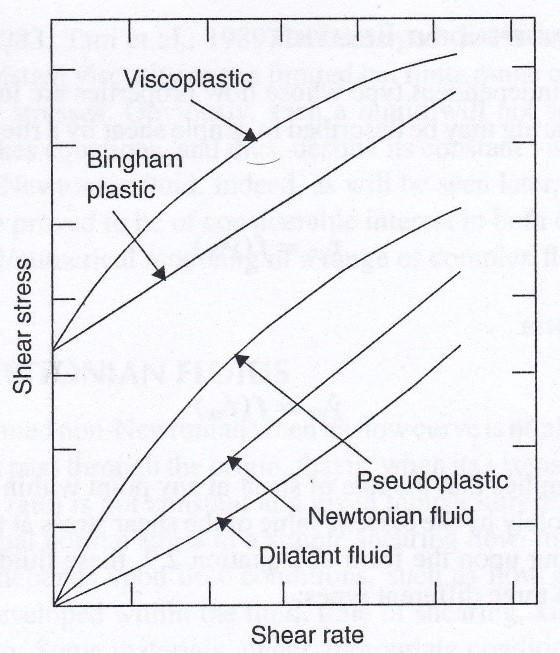
\includegraphics[width=8.0cm,clip]{1-Background/1-fluid-curve.jpg}
        \caption{Qualitative flow curves for different types of non-Newtonian fluids\cite{ref:1}.}
        \label{fig:1-fluid-curve}
        \centering
        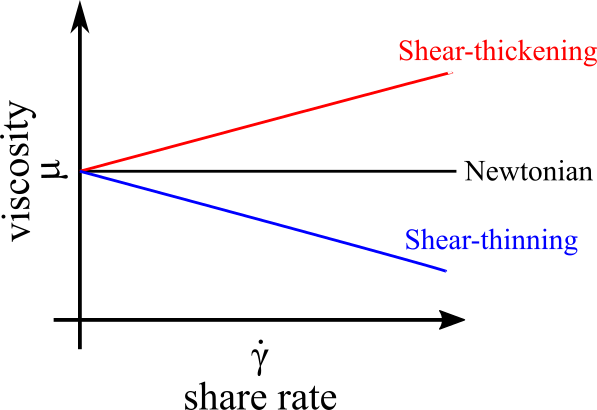
\includegraphics[width=8.0cm,clip]{1-Background/2-Newton-fluid.png}
        \caption{Classifications of non-Newtonian fluid.}
        \label{fig:2-Newton-fluid}
    \end{figure}

    \newpage
    \begin{figure}[h]
        \centering
        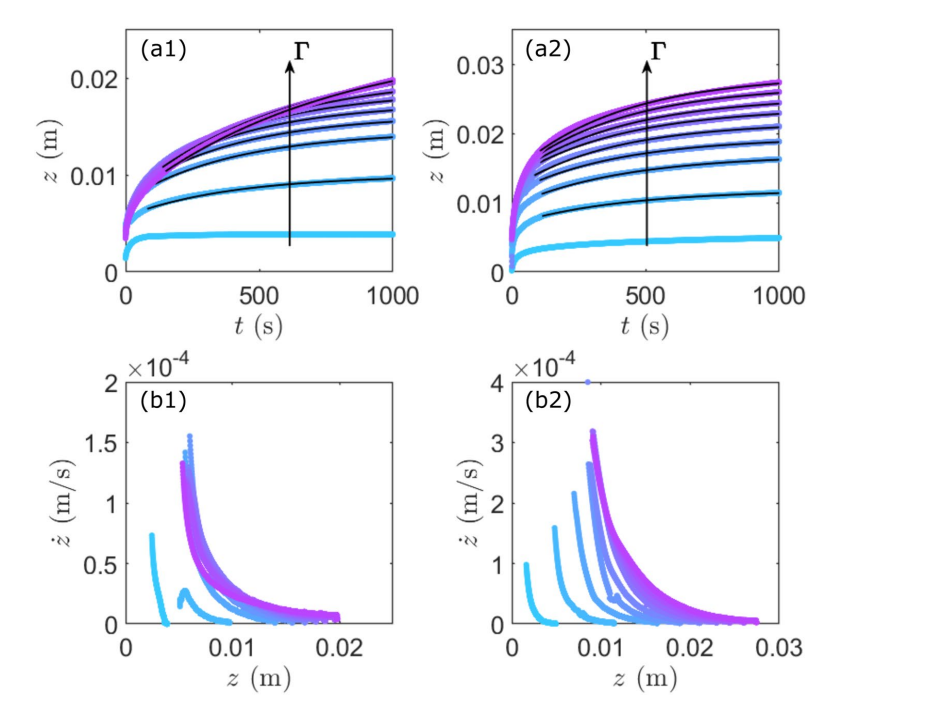
\includegraphics[width=11.0cm,clip]{1-Background/4-sinking.png}
        \caption{Sinking dynamics for different intruder-sizes and for different vibration intensities $\Gamma$. (a1) Depth versus time for an intruder with R=4mm and (a2) for an intruder with R=7mm. (b1) Instantaneous velocity versus sinking depth obtained from (a1) and (b2) from (a2). The black lines correspond to the solutions fitted in the quasi-steady regime\cite{ref:6}.}
        \label{fig:4-sinking}
    \end{figure}
\end{center}

\subsection{研究目的}

先行研究\cite{ref:8}において,落下球の把持を行うのに電磁石を用いていた.しかし,電磁石を用いた方法では強磁性体のみを把持することができ,それ以外の材質のものは把持することはできない.そこで落下球を把持する方法を,真空ポンプを用いて吸引する手法に変化させ実験を行った.この把持する手法の変化に伴い生じる,擬塑性流体中を落下する球への落下速度への影響について調査することを一つ目の目的とする.また異なる実験手法を用いることで,先行研究において生じている落下開始時のオーバーシュートに関してその要因を調査することを二つ目の目的とする.

また従来,球を落下させる試行ごとの間隔を10分と統一して行っていた.先行研究\cite{ref:8-5}にて,等間隔の時間で物体を落下させると,落下速度が一定になることが報告されているためである.これは落下球によって擬塑性流体の分子構造がせん断されたのちに回復するためである.一方で,試行ごとの落下間隔を変化させると,分子構造の回復割合が変化し,粘弾性特性が変化すると考えられる.このことによって発生する超音波照射による高速化への影響を調べることを三つ目の目的とする.
